\documentclass[11pt, a4paper]{MATH2023}
\usepackage{fancyhdr}
\usepackage{setspace}
\usepackage{amsmath,mathrsfs}
\usepackage{multicol}
\usepackage{amssymb}
\usepackage{graphicx}
\usepackage{caption}
\usepackage{subcaption}
\usepackage{xcolor}
\usepackage{enumitem}
\usepackage{tikz}
\usepackage{mathtools}
\usetikzlibrary{matrix}
\usepackage[normalem]{ulem}
\usepackage{multirow}
\usepackage[linesnumbered, ruled, boxed]{algorithm2e}
\SetKwRepeat{Do}{do}{while}
\newcommand{\eg}{\textbf{[Example.] }}
\newcommand{\sol}{\textbf{[Solution.] }}
\newcommand{\ii}{{\bf i}}
\newcommand{\jj}{{\bf j}}
\newcommand{\kk}{{\bf k}}
\newcommand{\rr}{{\bf r}}
\newcommand{\FF}{{\bf F}}
\renewcommand{\div}{{\rm div\ }}
\newcommand{\curl}{{\rm curl\ }}
\newcommand{\pt}{\partial}


\title{Chapter 13}
\subtitle{Application of Partial Derivatives}

\begin{document}
\begin{spacing}{1.3}

    \section{Extreme Values}
    {\blue Recall that in single variable calculus:

    $x_1$ is a {\it relative} maximum point, if $f'(x_1)=0$ and $f''(x_1)<0$,\\
    $x_2$ is a {\it relative} minimum point, if $f'(x_2)=0$ and $f''(x_2)>0$.
    }

    Similarly, in multi-variable calculus, the {\bf critical point} is where 
    \begin{center}
        \boxed{$$\disp \nabla f(\rr_0)=(f_{x_1}(\rr_0), f_{x_2}(\rr_0),\cdots,f_{x_n}(\rr_0))={\bf 0}$$}
    \end{center}
    

    And, if $h$ has a {\bf relative extremum} at a point $\rr_0$, then $\rr_0$ is a {\bf critical point},
    and $\nabla f(\rr_0)={\bf 0}$.
    However, if $\rr_0$ is a critical point, we {\it cannot infer} that $\rr_0$ is a relative extremum.
    The reason is similar in single variable calculus.

    \vspace{0.4in}
    Different from single variable, a critical point which {\it is not a relative extremum} can be 
    a {\bf maximum point, minimum point, } or a {\bf saddle point}.
    \begin{center}
        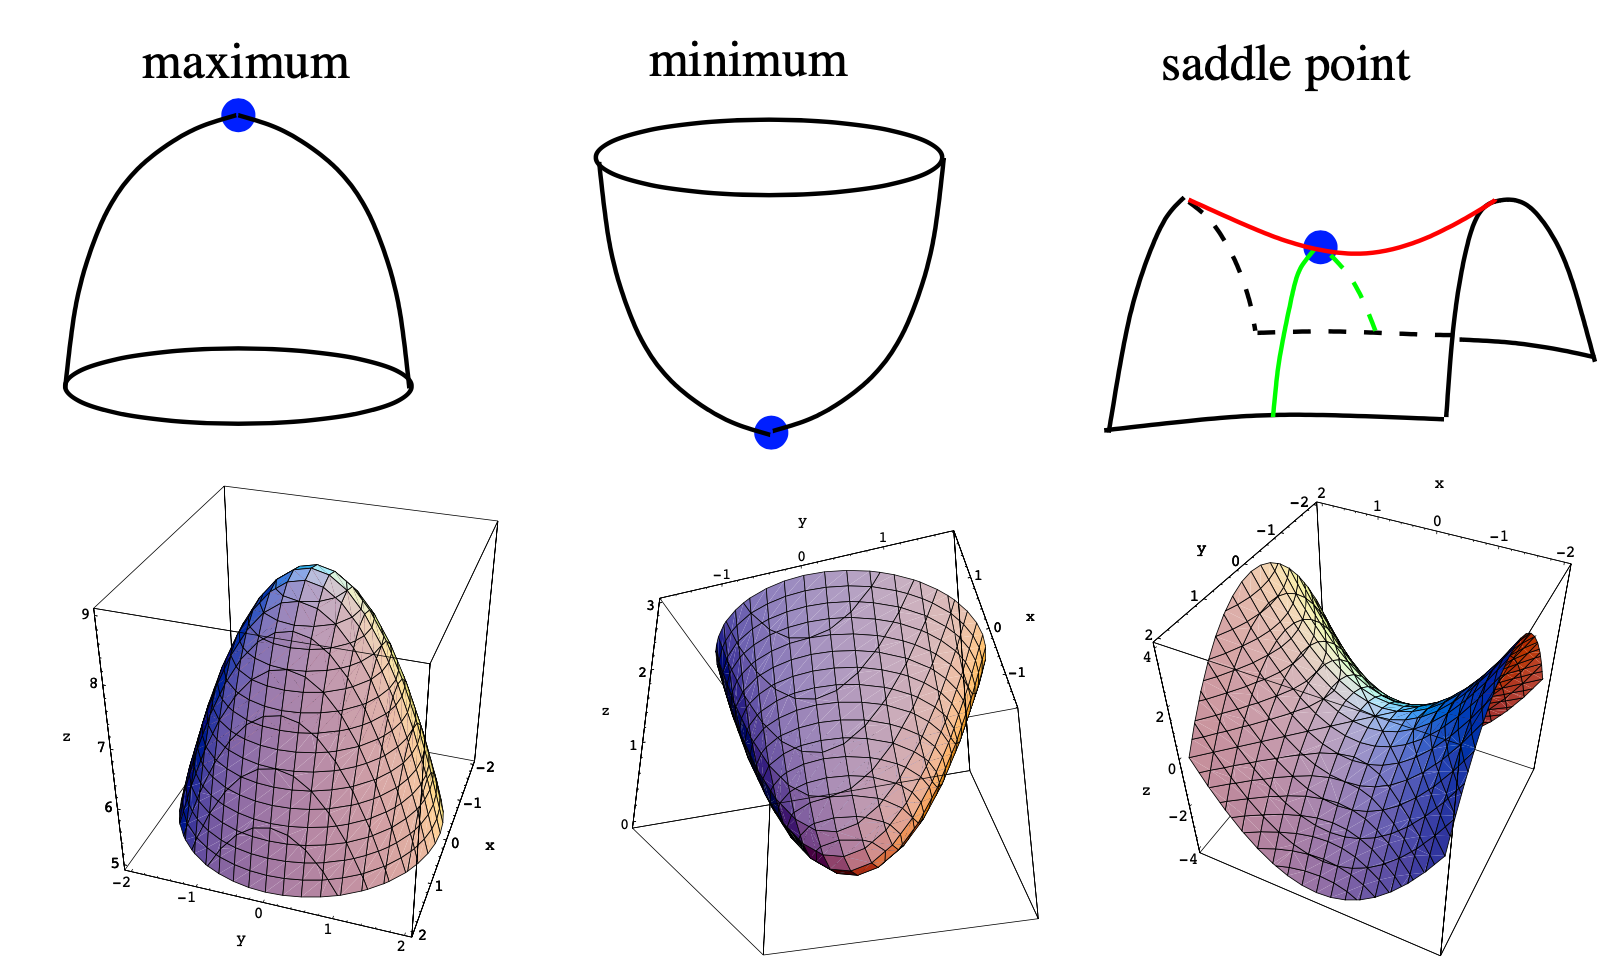
\includegraphics[scale=0.4]{images/Ch13-saddle.png}
    \end{center}

    \newpage
    However, to classify the critical points, we need the {\bf second derivative test}, or {\bf D-test}.

    \vspace{0.3in}
    {\bf Second Derivative Test}

    Suppose $f(x, y)$ has a critical point at $\mathbf{r}_{0}=\left(x_{0}, y_{0}\right)$ 
    (i.e. $\left.\nabla f\left(\mathbf{r}_{0}\right)=\mathbf{0}\right)$ and the second partial 
    derivative of $f(x, y)$ are continuous in a disk with center $\mathbf{r}_{0}=\left(x_{0}, y_{0}\right) .$ Let
    \begin{center}
        \boxed{$$\disp 
        D=\left|\begin{array}{ll}
        f_{x x}\left(\mathbf{r}_{0}\right) & f_{x y}\left(\mathbf{r}_{0}\right) \\
        f_{y x}\left(\mathbf{r}_{0}\right) & f_{y y}\left(\mathbf{r}_{0}\right)
        \end{array}\right|=f_{x x}\left(\mathbf{r}_{0}\right) f_{y y}\left(\mathbf{r}_{0}\right)-f_{x y}^{2}\left(\mathbf{r}_{0}\right)
        $$}
    \end{center}
    
    \begin{center}
        \begin{tabular}{c|c|c}
            \hline\hline 
            $D$ & $f_{x x}\left(\mathbf{r}_{0}\right)$ or $f_{y y}\left(\mathbf{r}_{0}\right)$ & nature of $\mathbf{r}_{0}$ \\\hline\hline
            $>0$ & $>0$ & relative minimum \\\hline
            $>0$ & $<0$ & relative maximum \\\hline
            $<0$ & & saddle point \\\hline
            $=0$ & & no conclusion can be drawn \\\hline
        \end{tabular}
    \end{center}
    
    \vspace{0.4in}
    {\it I'd like to omit the proof of D-Test here.}

    \vspace{0.8in}
    {\blue This example shows basic use of D-Test.}

    \eg Find the relative minima and maxima of $f(x, y)=x^{3}+y^{3}-3 x-12 y+20$.
    $$
    f_{x}=3 x^{2}-3 \quad \text { and } \quad f_{y}=3 y^{2}-12
    $$

    \sol 
    For critical points, $f_{x}=f_{y}=0 \quad \Rightarrow \quad x=\pm 1, y=\pm 2$.

    $\therefore (1,2),(-1,2),(1,-2),(-1,-2)$ are critical points.

    To apply D-Test, compute:
    $f_{xx}=6x, f_{yy}=6y, f_{xy}=0$, hence $D=f_{xx}\cdot f_{yy}-(f_{xy})^2= 36xy$

    \begin{center}
        \begin{tabular}{c|c|c|c|c|c}\hline\hline
            Point & $f_{xx}$ & $f_{yy}$ & $f_{xy}$ & $D$ & Type\\\hline\hline
            $(1,2)$ & 6 & 12 & 0 & 72 & min \\\hline
            $(-1,2)$ & $-6$ & 12 & 0 & $-72$ & saddle\\\hline
            $(1,-2)$ & 6 & $-12$ & 0 & $-72$ & saddle\\\hline
            $(-1,-2)$ & $-6$ & $-12$ & 0 & 72 & max\\\hline
        \end{tabular}
    \end{center}



    \newpage
    {\blue This example shows how to find extrema on a {\it closed} and {\it bounded} region.}

    \eg Find the absolute extrema of the function
    $$z=f(x, y)=x y-x-3 y$$
    on the {\it closed} and {\it bounded} set $R$, where $R$ is the triangular 
    region with vertices $(0,0),(0,4)$ and $(5,0)$.

    \sol $f_x=y-1, f_y=x-3, f_{xy}=f_{yx}=1, f_{xx}=f_{yy}=0, D=-1$

    For critical points, $\nabla f=(f_x, f_y)=(0,0) \Rightarrow x=3, y=1$.

    This point is inside the domain. But we still need to find possible 
    extreme points {\it on the boundary of domain}.

    {\bf (1)} Along $OA:$, $\rr_0=(0,0), \rr_1=(5,0)$, so the parametric representation 
    of line $OA$ is:
    $$\rr(t)=(1-t)\rr_0+t\rr_1,=(5t, 0),\ t\in [0,1]$$
    hence $z=f(\rr(t))=-5t,\ t\in [0,1]$

    So along $OA$, the possible extreme points are $(0,0)$ and $(5,0)$.

    {\bf (2)} Along $OB:$, similarly, $\rr(t)=(0, 4t),\ t\in [0,1]$, 
    $z=f(\rr)=-12t$,

    So along $OB$, the possible extreme points are $(0,0)$ and $(0,4)$.

    {\bf (3)} Along $AB:$ $\rr(t)=(5-5t, 4t),\ t\in [0,1]$,
    $z=-20t^2+13t-5,\ t\in [0,1]$

    There is one critical point on $AB$, when $dz/dx=0$, at $\left(\dfrac{27}{8}, \dfrac{13}{10}\right)$.

    Then we compute the value of all possible extremum points,
    \begin{center}
        \begin{tabular}{c|c}\hline\hline
            $(x,y)$ & $f(x,y)$ \\\hline\hline
            $(3,1)$ & $-3$\\\hline
            $\left(\dfrac{27}{8}, \dfrac{13}{10}\right)$ & $-\dfrac{231}{80}$\\\hline
            $(0,0)$ & 0 \\\hline
            $(5,0)$ & $-5$ \\\hline
            $(0,4)$ & $-12$ \\\hline
        \end{tabular}
    \end{center}

    Therefore, absolute maximum value is 0 which occurs at $(0,0)$,
    absolute minimum value is $-12$ which occurs at $(0,4)$. 


    \vspace{0.2in}
    {\blue This example converts the problem to max/min problem.}

    \eg Find the points on the surface $z^2=xy+1$ that are closest to the origin.

    \sol $d^2=(x-0)^2+(y-0)^2=x^2+y^2+xy+1=f(x,y)$, only need to minimize this function.


    \newpage
    \section{Lagrange multipliers}

    {\blue Motivation: sometimes we want to maximize/minimize $f(x,y)$ subject to $g(x,y)=k$.}

    {\bf How to find the maximum or minimum value?}
    \begin{enumerate}
        \item Find all values of $\mathbf{r}$ and $\lambda$ such that
        $$\nabla f(\mathbf{r})=\lambda \nabla g(\mathbf{r})$$
        and $$g(\mathbf{r})=k$$
        \item Evaluate $f$ at all the points $\mathbf{r}$ that arise from step (1). 
        The largest (smallest) of these values is the maximum (min) value of $f$.
    \end{enumerate}

    {\it \textbf{Remark:}} Lagrange's method only finds critical points, 
    it {\it does not tell} whether the function is maximized or minimized.

\end{spacing}
\end{document}
